\newpage
\section{Mining Scenario}

We present a model of a generalized scenario of the extractive area in underground copper mines, based on observations and procedures from El Teniente Division of Codelco. First, we analize the extractive process and environment in the mines; then the real scenario and mobility are described, concluding with abstractions and generalizations that allows us to have an accurate model of the extractive area of underground copper mines in Chile.

\subsection{The extraction process at El Teniente}

El Teniente Division is the biggest underground copper mine in the world, with a conical shape 3 km long, 1.5 km wide and around 1.8 km tall. The Braden formation is localized in the center of the ore body, shaped as an inverted cone with a 1.2 km surface diameter. The main infrastructure of the mine (main transfer shafts, primary crushers, and maintenance workshops) are located in the Braden formation at different depths, which contain small amounts of copper. The exploitation occurs around this formation, where the mineralization gave place to 3 different zones:

\begin{itemize}
    \item Sterile overload: Located on the top of the deposit, the overload consists of different copper oxides, considered sterile since El Teniente only exploits sulfides.
    \item Secondary mineralization: Located under the overload, the secondary mineralization is a rich zone with a copper content of approximately $1.8\%$. This rock is easily fragmented, so the Block Caving method with manual extraction and gravitational transfer can be used.
    \item Primary mineralization: Located under the secondary ore, the primary mineralization shows an important $50\%$ decrease in copper content, and is defined as hard rock with high friability. This requires a mechanization of the extraction process, using Block Caving with Load, Haul, Dump machines (LHDs) for extraction. Though this area is more expensive to exploit, its massive extension–running over 1000 m below the lower level of El Teniente (Teniente 8)–makes it one of the largest copper reserves in the world.

\end{itemize}

Currently, the extraction takes place in the primary mineralization, therefore LHDs are a necessity in the extracting area. Block Caving methods are primarily used to orchestrate the process. 

\emph{Block Caving} is a mining method used to excavate massive orebodies with high friability. In this process, a haulage access is made by undercutting the area below the orebody. Ore between the undercut and haulage level is removed at strategic locations, which then serve as extraction points for further excavation. The orebody is drilled and blasted above the undercut, and the ore is removed by the LHDs using the haulage access. As ore is removed from the drawbells, the orebody sinks, providing a continuous stream of ore. If the caving stops but the removal of ore continues, a large void may form, which has the potential for a sudden, massive collapse.

The ore, despite its high friability, generally fragments into various sizes which range from 1 mm to over 1 m in diameter. A crushing process further reduces all rock to 13 mm or less. The uniform fragments are then grinded to 180 microns, which can be used in the flotation process to obtain the copper concentrate.

The ore carried by the LHDs is thrown into a shaft through a strainer, where big rocks can be hammered to obtain a diameter under 1 m. Gravity moves these rocks to the primary crushing process, executed both inside and outside of the mines, which reduce the size of the rocks to 20 cm. The rest of the crushing is completed on the outside, carrying the ore using conveyor belts to the crushing plant. 


\subsection{Communication Requirements}

Underground mining is one of the most extreme occupations from several perspectives. The mining operations are carried out in hazardous environments. The risk of roof falls, explosions, floods, etc., can cause accidents resulting in fatalities, especially when emergency response tends to be slow and difficult in remote areas where mines are generally stationed. Nevertheless, efficiency and productivity must always be maintained during mining operations.

Communication is indispensable to maintain a safe environment in a highly efficient production, and is used in every stage of the mining operations. Extraction and transport of the ore is handled with the aid of communication, increasing productivity in tasks that require perfect synchronization. Remote activities, such as monitoring and control, heavily rely on communications. In emergency conditions, communication is of vital importance, providing an information flow which includes coordination and localization of workers. In the last few decades, radio communication in mines has been an important issue across the world, where tests have been carried out to determine best results (see Annex 1), still not providing a definitive answer [5].


\subsection{Extraction process}

El Teniente Division is the biggest underground copper deposit in the world, with a conical shape 3km long, 1.5 km wide and around 1.8km tall. In the center of the ore body the Braden formation is localized, shaped as an inverted cone with a 1.2km diameter on the surface. All the main infrastructure of the mine, such as shafts, main transfer shafts, primary crushers, and maintenance workshops, are located in the Braden formation in different levels. This area have a small amount of copper. All mines operate around this, as it can be seen in \ref{fig:teniente}.

\begin{figure}
    \centering
    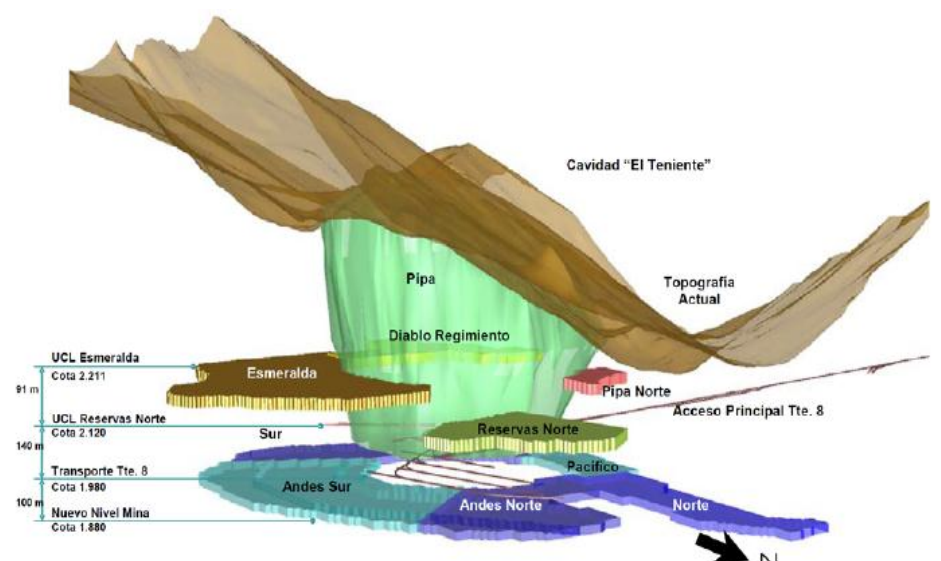
\includegraphics[width=400pt]{img/teniente.png}
    \caption{3D view of the different levels and mines in El Teniente Division \cite{baraona}}
    \label{fig:teniente}
\end{figure}


The exploitation occurs around this formation, where the mineralization gave place to 3 different zones:
\begin{enumerate}
    \item \emph{Sterile overload:} Located on the top of the deposit, it consists of different copper oxides, considered sterile since El Teniente only exploits sulphurs. 
    \item \emph{Secondary mineralization:} Located under the overload, it's a rich zone with a copper content of approximately $1.8\%$. This rock is easily fragmented, so the Block Caving method with manual extraction and gravitational transfer can be used.
    \item \emph{Primary mineralization:} Located under the secondary ore, it shows an important $50\%$ decrease in its copper content, and is defined as hard rock. This requires a mechanization of the extraction process, using Block Caving with LHDs (\emph{Load Haul Dump} machines) for extraction. Though this formation is more expensive to exploit, its big extension -running over 1000m below the lower level of El Teniente (Teniente 8)- makes it one of the biggest copper reserves in the world.
\end{enumerate}

The current extraction takes place in the primary mineralization, therefore LHDs are a necessity in the extracting area. To orchestrate the process, Block Caving and Panel Caving methods are used to 



\subsection{Scenario and mobility}

The scenario of an underground mine depends very much on the 

\subsection{Hypothesis and Generalizations}

\subsection{Extractive area model}





En este caso, consideraremos principalmente el nivel de extracción de una mina, donde se cuenta con vehículos que ingresan y salen del área cívica. Estos vehículos constan de acumulaciones de nodos, pero también son un nodo en sí mismos.

Luego de dejar a los otros nodos, los vehículos se van. Se tiene el centro cívico, que es el lugar donde los supervisores salen a dar rondas, y de donde todos los nodos, excepto los LHDs, van y vuelven.

La jornada de trabajo consiste en tener supervisores que dan rondas, y operarios que manejan las máquinas realizando circuitos entre el área de explotación y el área de chancado primario.

Consideraremos también grupos de mineros que van a puntos particulares del mapa, trabajan ahí en un rango pequeño, y luego vuelven al centro cívico.

Así podemos adaptar el escenario de desastre tal que tengamos las siguientes zonas:

Entrada al centro cívico
Interior centro cívico: 
Explotación: movimiento circular de las máquinas, rápidas (Nstat), movimiento aleatorio de nodos desde el centro cívico (.
Mantenimiento: La gente va, se queda ahí un rato, vuelve al centro cívico.

Para simular escenarios de minería, tomaremos como referencia el modelo de desastre 


\section*{Mining Scenario}

El siguiente escenario propone 

Zonas: OT, CC, OP, PR
Nodos: personas, vehiculos, LHDs
Tipo: transporte, estáticos


